\documentclass{beamer}
\usetheme{Berlin}
\setbeamercovered{dynamic}
\usepackage{lipsum}  
\usepackage{hyperref}
\usepackage{colortbl}

\title[Assignment]{Assignment}
\subtitle{CS 213, Software Systems Lab}

\author{Sakeena Dodda \\
  Computer Sciene and Engineering \\
  210010062@iitdh.ac.in}
  \logo{
\includegraphics[width=1.3cm,height=0.391cm]{logo.png}}
\institute[CSE, IIT Dharwad]{Indian Institute of Technology, Dharwad}
\date{\today}

\begin{document}
\frame[plain]{\titlepage}
\begin{frame}[label=page_2]
Hello, This is our first frame. Here, you can find information about IIT Dharwad at the below mentioned link: \url{www.iitdh.ac.in} or by clicking the following name: \href{http://www.iitdh.ac.in}{IIT Dharwad}
\\
You can find info about Super Heroes by clicking the following button: \hyperlink{page_22}{\beamergotobutton{Super Heroes}}

You can find info about mathematicians by clicking the following button: \hyperlink{page_21}{\beamergotobutton{Mathematicians}}
\end{frame}

\section[Structures]{Structures}
\begin{frame}
\frametitle{Structures}
\only<1>{
  \begin{block}{Theorem : Magic}
My name is Alt Temporal. I can do magic by changing myself in different slides.
\end{block}
\begin{alertblock}{The Truth }
No, don't trust him, he doesn't do magic.
\end{alertblock}
}
\only<2>{
 \begin{block}{Theorem : Magic}
I have done the magic. You should have trusted me earlier before I have done the magic.

\end{block}
\begin{alertblock}{The Truth }
I was just joking, The above person actually does the magic and also I can do it.
\end{alertblock}
}
\end{frame}


\begin{frame}{Structures with columns}
\begin{columns}
\column{0.4\textwidth}
\begin{alertblock}{Alert Column}
Remain alert for the red light.
\end{alertblock}
    
\uncover<3->{
\column{0.4\textwidth}
    \begin{exampleblock}{To Go}
    Green light means to go past.
    \end{exampleblock}
    }
\end{columns}

 \begin{columns}
 \uncover<2->{
 \column{0.4\textwidth}
        \begin{block}{Test your Skills}
    There won’t be any blue light at the signal.
    \end{block}
    }
\uncover<4->{
\column{0.4\textwidth}
\begin{exampleblock}{Extra Info}
    Green is also the color of this example block.
    \end{exampleblock}
    }
\end{columns}
\end{frame}
   
\section{Tables}

\begin{frame}{Table Frame 1}
    \begin{table}[h]
     \centering
      \begin{tabular}{c c c}
        \hline
        Our Sir in Google Meet  & Student A &   \pause \\
              & Student B &  \pause \\
        \hline
             Student C & Student D & Student E\\
        \hline
        \end{tabular}
\caption{ Google Meet Interface as a Table with Teacher}
\label{Table:}
 \end{table}
The table number shows teacher interacting with students in
Google Meet interface.
\end{frame}

\begin{frame}{Table Frame 2}
\begin{table}[h]
    \centering
    \begin{tabular}{c c}
    \hline
        \multicolumn{2}{c}{Students} \\
        A & B \\
        \hline
    \end{tabular}
    \caption{Google Meet Interface as a Table without Teacher}
    \label{tab:mylabel}
\end{table}
The table number shows students in Google Meet interface.
    
\end{frame}

\begin{frame}{Table Frame 3}
    \begin{table}[]
    \centering
     \caption{My Sample Table}
     \begin{tabular}{l|c|c|c}
\textbf{Value 1} &\textbf{Value 2}  & \textbf{Value 3} & \textbf{Value 4}\\ \hline
            1& 5 & 6 &8 \pause\\
            2 & 9  & 11 & 13  \pause\\
             3&  58 & 23  & 62\\
\end{tabular}
\label{tab:my_label}
\end{table}
\pause  
This is a sample table consisting of random things
\end{frame}

\begin{frame}{Table Frame 4}
\begin{table}[]
\centering
\caption{Students and their Marks}
\begin{tabular}{lc<{\onslide<2->}c<{\onslide<3->}c<{\onslide<4->}c<{\onslide}c}
Sub & A & B & C & D \\
  Mat     & 35 & 62 & 93 & 34 \\
  Phy     & 32 & 41 & 56 & 96 \\
  Chem    &55&83&58&92
\end{tabular}
\end{table}
\end{frame}

\section{Transitions}

\begin{frame}{Transition 1}
\lipsum[1-1]
\end{frame}
\begin{frame}{Transition 2}
\lipsum[2-2]
\end{frame}
\begin{frame}{Transition 3}
\lipsum[3-3]
\end{frame}
\begin{frame}{Transition 4}
\lipsum[4-4]
\end{frame}

\section{Figures}
\begin{frame}{Great Mathematicians}
This frame shows pictures of Great Mathematicians.
\begin{columns}
\hspace{2.4em}
\begin{column}{0.31\textwidth}
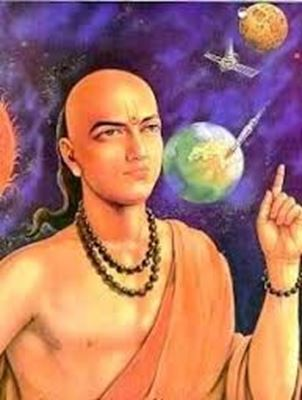
\includegraphics[scale=0.4]{aryabhatta.jpeg}
\end{column}
\begin{column}{0.8\textwidth}
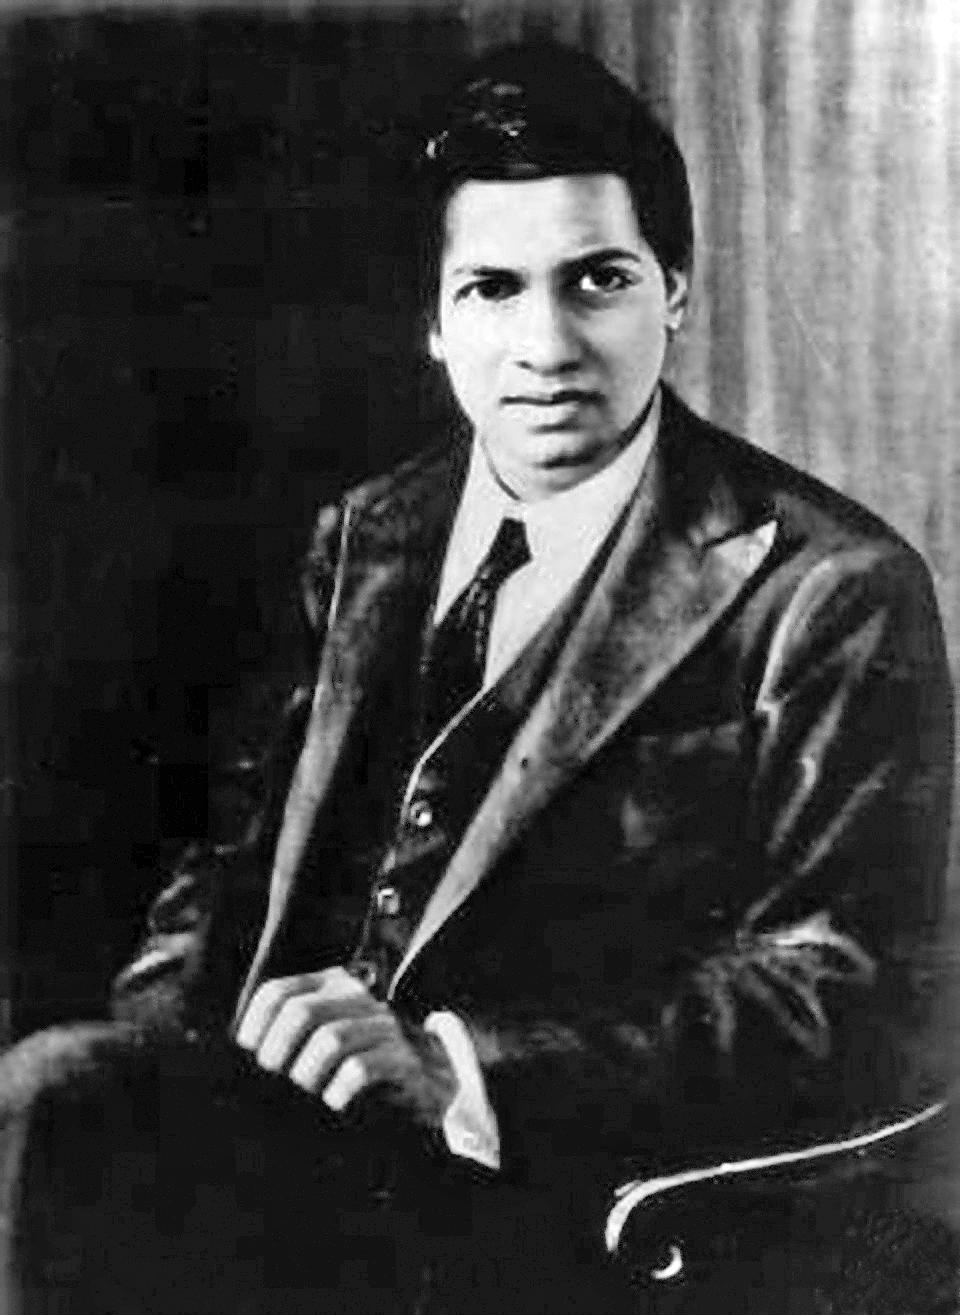
\includegraphics[scale=0.09]{Srinivasa.jpg}
\end{column}
\end{columns}   
\end{frame}

\section{Mathematics}
\begin{frame}{Mathematics}
    Mathematics is a subject that we learn in the class. This is what you may have known. But it’s something else. It’s a world of numbers.\\
    \pause
    Mathematics consists of \\
    1) Theorem or Proofs \pause\\
    2) Equations\\
    \invisible<1-2>{This is the last slide of Mathematics Intro}
    
\end{frame}

\begin{frame}{Theorems or Proofs 1}
    \begin{block}{Theorem: The Most Complicated One}
        $(a+b)^2=a^2 + b^2 + 2ab$
    \end{block}
    \begin{exampleblock}{Proof:}
    \begin{eqnarray}
            (a+b)^2 & = & (a+b)(a+b) \nonumber \\
                    & = & a^2 + ab + ba + b^2\nonumber \\
                    & = & a^2 + b^2 +2ab\nonumber
    \end{eqnarray}
    \end{exampleblock}
\end{frame}

\begin{frame}{Theorems or Proofs 2}
    \begin{block}{Theorem: The Second Most Complicated One}
        $(a-b)^2=a^2 + b^2 - 2ab$
    \end{block}
    \begin{exampleblock}{Proof:}
        \begin{eqnarray}
            (a-b)^2 & = & (a-b)(a-b) \nonumber \\
                    & = & a^2 - ab - ba + b^2\nonumber \\
                    & = & a^2 + b^2 -2ab\nonumber
    \end{eqnarray}
    \end{exampleblock}
\end{frame}

\begin{frame}{Theorem Other Way}
    \begin{block}{Theorem}
        $Multiplication \; is \; not \; Commutative\; in\; Matrices.$
    \end{block}
    \begin{block}{Proof.}
        AB is not equal to BA.
    \end{block}
\end{frame}

\begin{frame}{Equation -1}
This frame will consist of a multiline equation as follows:\\
Our Multiline Equation:\\
Area of Circle
\begin{eqnarray}
            A & = & \pi r^2  \pause\\ 
              & = &\frac{\pi d^2}{4}\nonumber 
\end{eqnarray}
\end{frame}

\begin{frame}{Equation -2}
This frame will consist of onemore multiline equation as follows:\\
Our Multiline Equation:\\
Einstein’s Equation
\begin{eqnarray}
            E & = & mc^2 \nonumber \\
    \only<2->{& = & (\sqrt{mc})^2 }\nonumber
\end{eqnarray}

\uncover<1-1>{See magic converts single line eqn to multi line eqn}\\
\only<2->{See I said no, I know magic, you should agree}
\end{frame}

\section{Our Section of Lists}

\begin{frame}{Our First List using itemize}
Hello\pause 
\begin{itemize}
    \item This is the first list item 
    \uncover<2->{\item This is the second list item}  
    \item This is the final list item which will be visible in all slides of
the frame
\end{itemize}

\end{frame}

\begin{frame}[label=page_21]{Our Second List using enumerate}
Well known famous People
\begin{enumerate}
    \item \href{https://en.wikipedia.org/wiki/Aryabhata}{Aryabhatta}\pause 
    \item \href{https://en.wikipedia.org/wiki/Albert_Einstein}{Einstein}\pause 
    \item \href{https://en.wikipedia.org/wiki/Newton}{Newton}\pause 
    \item \href{https://en.wikipedia.org/wiki/Niels_Bohr}{Bohr}\\
    You can find more info about them by clicking on their names
or by searching at Google
\end{enumerate}
\end{frame}

\begin{frame}[label=page_22]{Our Third List using Description}
\begin{description}
    \uncover<2->{\item[Iron Man] His speciality is he wears a iron man suit.}
    \uncover<3->{\item[Thor] He has a hammer.}
    \item[Vivek] He know’s how to use Beamer.
\end{description}
\alert<3>{Hereby all our lists are also completed}
\end{frame}

\begin{frame}{Our Final Frame that has Different Slides}
\color<1->{blue}{This frame is dedicated to the Beamer and people of IIT Dharwad
who are using it.}\\
\alert<1->{This is our final frame, and it says that all the given tasks are
completed by:}\\
\color<1->{blue}{To go back to the first frame after title click the following button.}\\
\hyperlink{page_2}{\beamerreturnbutton{Our First Frame}}
\pause
\end{frame}

\end{document}
